\documentclass[12pt]{book}

\usepackage[toc]{appendix} % para crear ambientes de apéndice
\usepackage{amsmath,amssymb, amsthm} % Para mejorar ecuaciones
\usepackage[utf8]{inputenc}
\usepackage[spanish]{babel} % Español
\usepackage[nice]{nicefrac}  % Para mejorar fracciones
\usepackage{graphicx} % Para insertar graficos
\usepackage{float} % Para manejar la ubicacion de graficos
\usepackage[colorlinks=true, allcolors=black]{hyperref} % Para hipervincular las referencias dentro del texto
\usepackage[Conny]{fncychap} % Capítulos

\usepackage{marginnote}% Paquete para notas al márgen
    \setlength{\marginparwidth}{4cm} % Ancho de la nota al margen
    \setlength{\marginparsep}{0.5cm} % Distancia mínima entre la nota y el texto principal
\usepackage{multirow,array}


\title{MICROECONOMÍA\\como una economía política}
\author{Oscar Landerretche\\Universidad de Chile}

\begin{document}

Este documento es una colección de apuntes de materia elaborados para armar el libro del ramo de Economía Política por el profesor Óscar Landerretche en la Facultad de Economía y Negocios de la Universidad de Chile. \\

Esta es una versión muy prematura del apunte por lo que puede contener errores. La última actualización se hizo en marzo de 2024, cualquier error por favor notificarme al correo, joamartine@fen.uchile.cl.

\maketitle        



%%%%%%%%%%%%%%%%%%%%%%%%%%%%%%%%%%%%%%%%%%%%%%%%%%%%%%%%%%%%%%%%%%%%%%

\newpage 

\setcounter{tocdepth}{1} % La tabla de contenidos solo llegará a mostrar hasta section
\tableofcontents

\chapter{Introducción}

\section{¿Qué es la economía política?}

En 1878, el filósofo y economista marxista Friedrich Engels publicó el segundo volumen la que es considerada como su mayor aporte a la teoría marxista de la época. Se titula \textit{Herrn Eugen Dühring's Umwälzung der Wissenschaft}, esto es ``La revolución científica del Señor Eugen Dühring'', un texto que se conoce como el ``Anti-Dühring''.\footnote{Engels, Friederich (1877/78) \textit{Herrn Eugen Dühring's Umwälzung der Wissenschaft. Philosophie, Politische Oekonomie, Socialismus}, Genossenschafts-Buchdruckerei, Leipzig, Imperio Alemán} En ése texto, escrito para refutar las tesis filosóficas y políticas de un rival de Karl Marx, quien se encontraba, en ese momento, demasiado ocupado trabajando en ``El capital.'' se ofrece la definición clásica de Economía Política: \\

\hfill\begin{minipage}{\dimexpr\textwidth-2cm}
``La economía política, en el sentido más amplio, es la ciencia que estudia las leyes que gobiernan la producción y el intercambio de los medios materiales de subsistencia en la sociedad humana... por lo tanto, la economía política es esencialmente una ciencia histórica. Se ocupa de material que es histórico y que está en constante cambio.''
\end{minipage}

\marginnote{\textbf{Economía política:} Definición}[0cm] % nota al margen, los cm del corchete es la distancia hacia abajo o hacia arriba de la nota con respecto a donde está escrito en el código. (2 cm hacia abajo [2cm], 2cm hacia arriba [-2cm])

\section{Microeconomía y macroeconomía}

\section{El problema de la racionalidad}

\chapter{Epistemología económica}

\section{El homo económico}

\section{Racionalidad limitada}

\section{Inferencia y comportamiento}

\section{Intuición y comportamiento}

\section{Trampas de ignorancia}

\chapter{El problema de lo privado y lo público}

\input{Tex/Economía descentralizada}

\section{Poder de mercado}

\section{Bienes club, comunes y públicos}

\section{Elección pública}

\section{Externalidades}

\subsection{Motivación}
Al abordar la temática de externalidades comenzamos a salir del marco walrasiano, si bien está es conocida como una falla de mercado clásica, es muy interesante estudiarla desde la economía política ya que existen distintas soluciones que se relacionan con tendencias ideologicas.

Consideramos como externalidad\footnote{Para efectos de este curso nos centraremos en la externalidades de equilibrio parcial.} la situación donde, ya sea la producción o consumo de un bien, tiene efectos en el bienestar de un tercero que no participa de la interacción de mercado. Entre los ejemplos típicos encontramos las externalidades ambientales, el caso del fumador, aumento de la educación, entre otros. Esta falla de mercado nos saca del marco walrasiano ya que desde el punto de vista social no tenemos un mercado en equilibrio.

\subsection{Externalidad en la producción}

Para analizar el funcionamiento de las externalidades negativas en la producción, utilizaremos como benchmark el equilibrio parcial de un mercado en competencia perfecta. Este modelo de mercado se compone por una oferta y demanda privada, las cuales en su interacción nos entregan un precio y una cantidad de equilibrio.

La oferta privada en este mercado está definida por el costo marginal de producción del bien ($Cmg$) percibidos por quien produce, estos pueden ser costos provenientes de la compra de insumos, gastos en energía, arriendo de un local, etc. 

\begin{figure}[h]
    \centering
    \caption{Equilibrio parcial en competencia perfecta}
    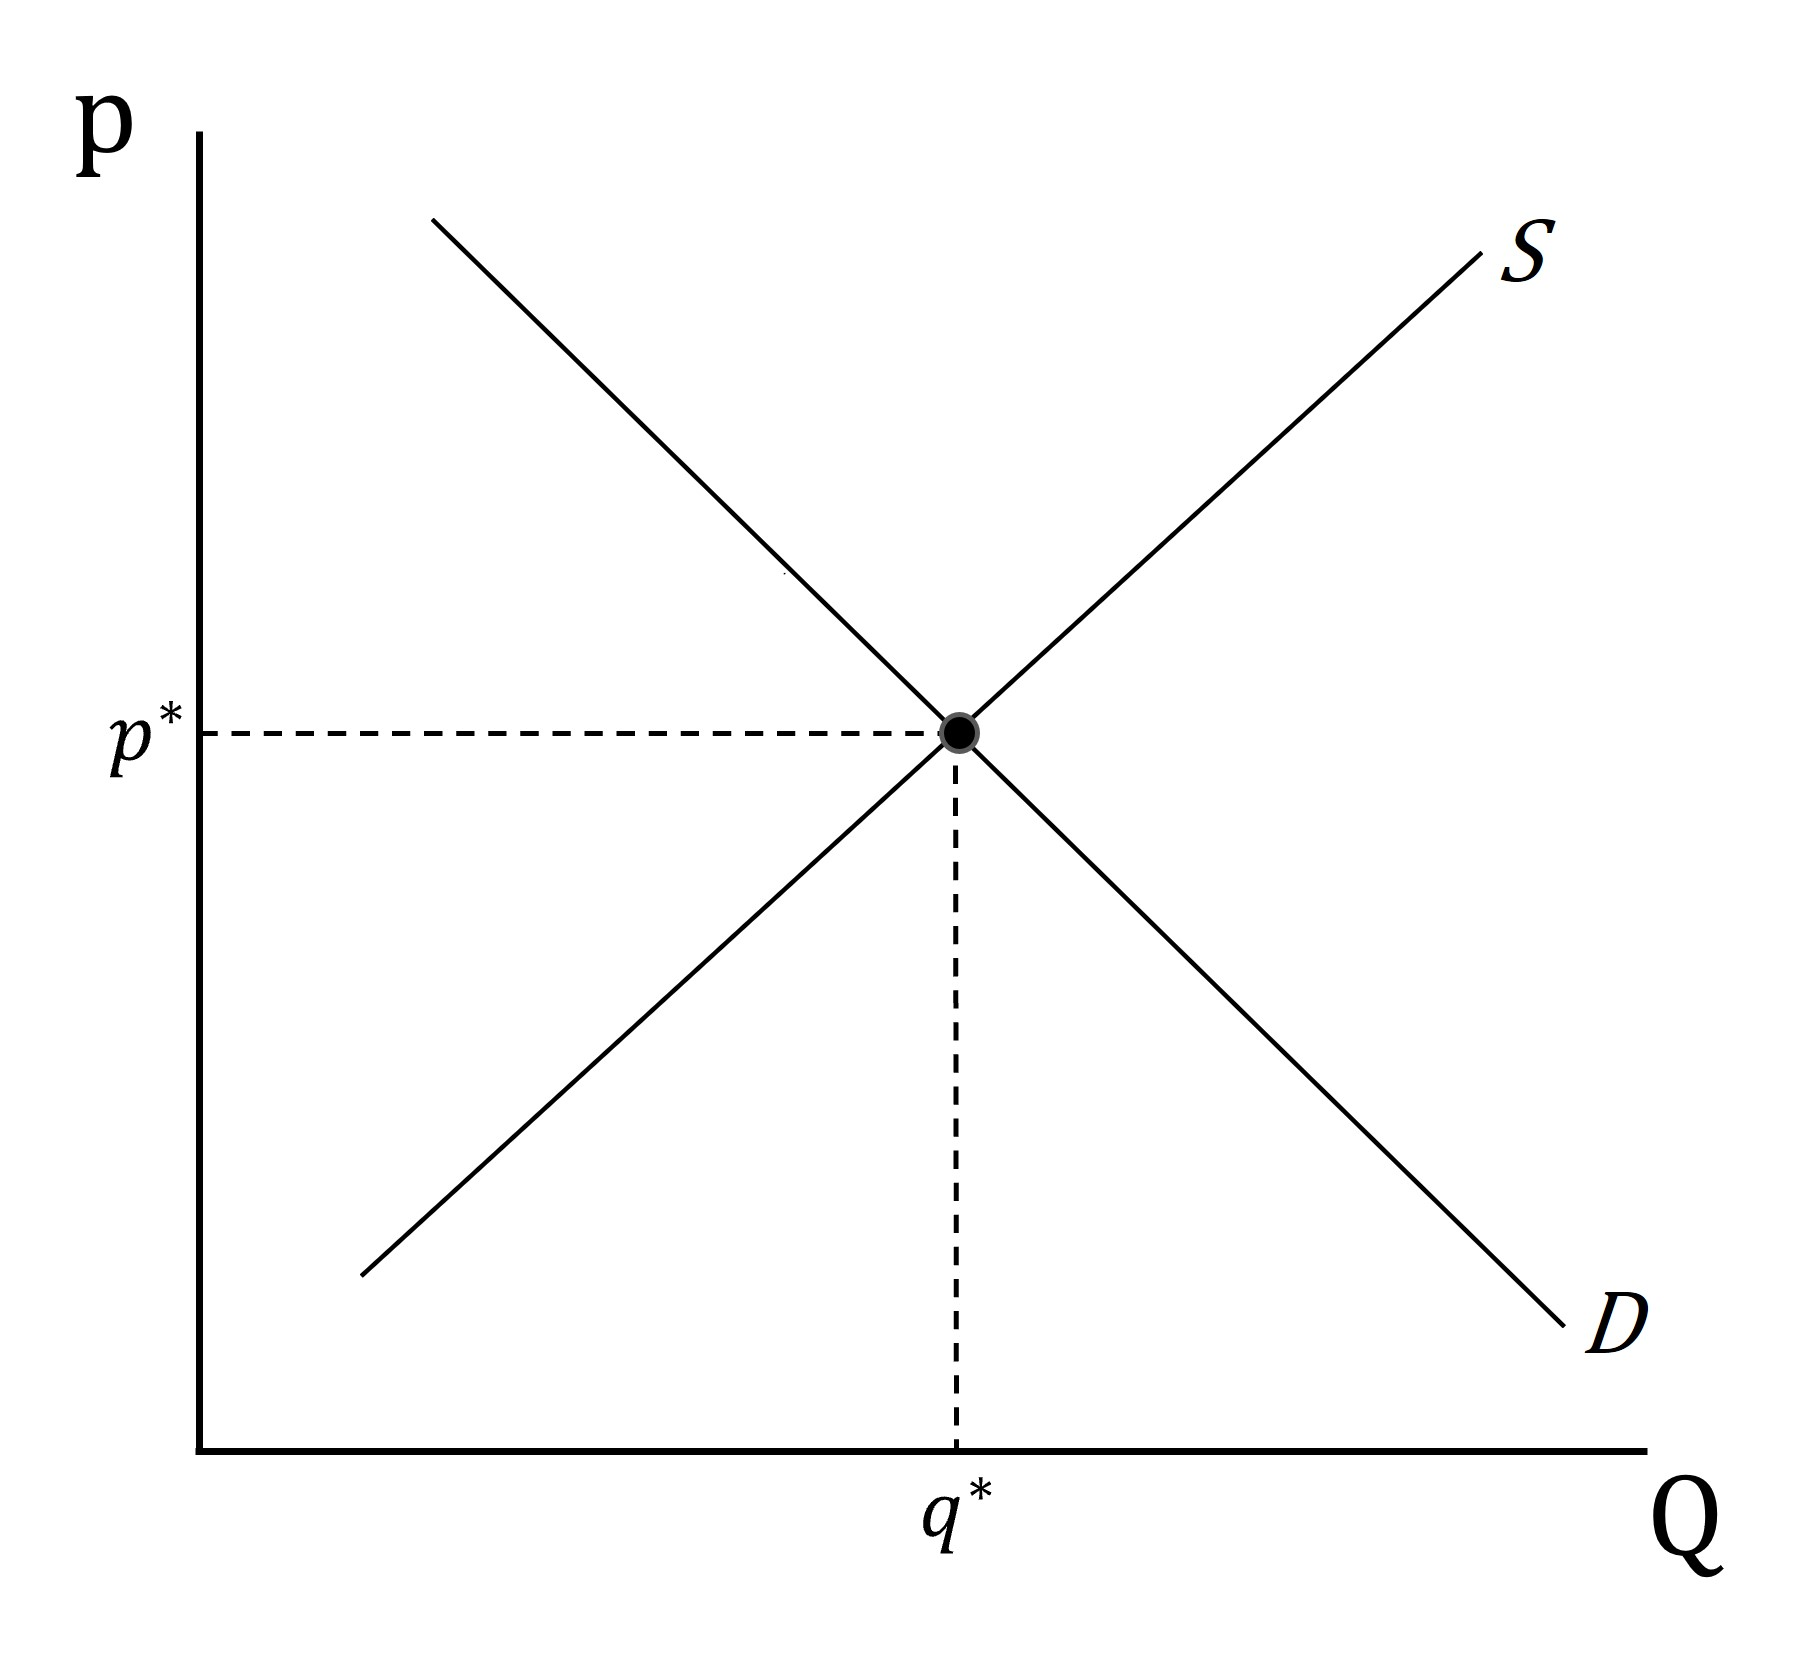
\includegraphics[width=0.5\textwidth]{Figuras/Eq Parcial EXT.jpg}
    \label{fig:Eq parcial}
\end{figure}

Para añadir externalidades negativas a este modelo, debemos considerar que existen costos adicionales que no son percibidos ni reconocidos por quién produce, por lo tanto tampoco son reflejados en la curva de oferta privada, estos nuevos costos los llamaremos ``costos sociales''. Con estos mayores costos, obtenemos que en equilibrio deberíamos observar un precio mayor y una cantidad producida menor.

\begin{figure}[h]
    \centering
    \caption{Externalidad en la producción}
    \includegraphics[width=0.5\textwidth]{Figuras/Externalidad Producción.jpg}
    \label{fig:Ext. Producción}
\end{figure}

\subsubsection{Externalidad en la demanda}

Para el caso de externalidades positivas el problema no radica en costos no considerados, sino que existe una demanda social que es mayor a la privada. Para analizar este tipo de externalidad nuevamente utilizaremos como benchmark el equilibrio parcial de un mercado en competencia perfecta.

Con lo anterior tenemos que la demanda privada representa la disposición a pagar por el consumo individual de un bien, esto genera que se subestimen los beneficios que tiene sobre la sociedad el consumo de dicho bien. Por otro lado, la demanda social si refleja de manera fidedigna los beneficios generados a nivel social por el consumo del bien, la internalización de estos beneficios resultaría en una mayor disposición a pagar.

El resultado del equilibrio en el mercado considerando la demanda social nos entrega un mayor precio y cantidad producida.

Las externalidades negativas tambien se pueden representar por el lado de la demanda, esto ocurre cuando el efecto en el bienestar del tercero viene dado por el consumo del bien más que por su producción, ejemplo de esto es el consumo del cigarro, con esto tenemos que quien consume no internaliza la desutilidad que genera en los demás agentes y por lo tanto no representa la disposición a pagar de la sociedad. El equilibrio del mercado resulta diferente para este caso, ya que tenemos que en equilibrio el precio y la cantidad producida disminuyen

\subsubsection{Solución Pública}

La solución de carácter pública para corregir esta falla de mercado fue creada por el economista \textbf{Arthur Pigou}\marginnote{\textbf{Arthur Pigou:}(1877-1959) Economista inglés de la Universidad de Cambridge, conocido por inventar el término \textit{externalidades} y contribuir con su solución pública.}, los mecanismos utilizados por esta solución los conocemos como \textit{impuestos y subsidios pigouvianos}, y los supuestos utilizados son que el estado tiene información completa acerca de las preferencias de la sociedad y además la capacidad suficiente para que sus impuestos o subsidios modifiquen el comportamiento de los agentes.

Es importante conocer la diferencia entre tipo de impuestos, de manera general en el estado encontramos impuestos utilizados con el fin de recaudar y subsidios que se enfocan en redistribuir, por otra parte tenemos los impuestos y subsidios pigouvianos que corrigen externalidades mediante un cambio en el comportamiento de los agentes. Dentro de los ejemplos clásicos de impuestos y subsidios pigouvianos encontramos el impuesto al tabaco y los colegios subvencionados.

\subsubsection{Medida de efectividad}

Para poder medir la efectividad de la solución pública utilizaremos como herramienta la \textit{evaluación social de proyectos públicos}, esta es un área de la economía desarrollada por \textbf{Arnold Harberger}\marginnote{\textbf{Arnold Harberger:}(1924-) Economista estadounidense de la Universidad de Chicago, conocido por ser pionero en el estudio de la evaluación social de proyectos públicos}. Considerando que la aplicación de impuestos o subsidios es costosa (Ej: costos de administración), la evaluación social consiste en comparar las preferencias sociales y privadas, para determinar la magnitud de la \textit{pérdida social}\footnote{En inglés se conoce como \textit{dead weight loss (DWL)}} existente en un mercado, representada gráficamente por los \textit{triángulos de Harberger}, con esto podremos comparar los costos y beneficios de resolver una externalidad y usar esto como medida de eficiencia. 

\section{Fallas del Estado}

\section{Trampas de ineficiencia y trampas de ineficacia}

\begin{appendices}
\chapter{Anexo}

\section{Demostración Ley de Walras}

Definimos el exceso de demanda como $\textit{q}(p)$ (ecuación \ref{eq: e demand}) considerando las demandas marshallianas de los bienes $x$ e $y$ y las dotaciones $\omega_x$ y $\omega_y$. Por notación dejamos las demandas marshallianas como $\xi_j$ siendo $j$ el conjunto de bienes, esto con el fin de generalizar la ecuación. 
\begin{equation}
     \textit{q}(p) =  \left[  \sum ^n _{j} \xi_j - \sum ^n _{j} \omega_j \right] \label{eq: e demand}
\end{equation}

Donde además diremos que para todo mercado $j$ se cumple la igualdad.
\begin{equation}
    \sum ^n _{j} p_j \xi _j(p,R) = \sum ^n _{j} p_j \omega_j \label{eq: eq de mercado}
\end{equation}

Para completar la demostración ponderamos el exceso de demanda por el vector $p$.
\begin{equation}
    p\textit{q}(p) = p \left[  \sum ^n _{j} \xi_j - \sum ^n _{j} \omega_j \right] = \sum ^n _{j} \left[ p_j \xi_j(p,R) - p_j \omega_j    \right] = 0
\end{equation}

Lo cual se debiera cumplir por la igualdad (\ref{eq: eq de mercado}). 


\section{Equilibrio General con Producción}
Habrá una dotación de factores productivos $K,L$ en donde habrá un total de $\bar{K}$ y $\bar{L}$ para cada factor respectivamente. Asumiremos la función Cobb-Douglas para la función de utilidad y de producción.  
\begin{align*}
    U_i (x_i,y_i) = x_i^\alpha y_i ^{1-\alpha},  \quad i = A,B \\
    x(K,L) = K_x^\beta L_x ^{1-\beta}, \quad y(K,L) = K_y^\beta L_y^{1-\beta}  
\end{align*}
Es decir que los dos individuos consumen los bienes $x,y$ producidos con los factores $K,L$. Las variables $\alpha$ y $\beta$ representan las preferencias y ponderaciones para el consumo y producción respectivamente. 

\subsubsection*{Curva de contrato de producción}

La eficiencia de producción se dará maximizando la producción de un bien sujeta a la producción del otro. De esta manera encontraremos los puntos que pertenecen a la frontera de posibilidades y que por tanto son eficientes. 
\begin{align*}
    \max _{K_x,L_x} \quad &x = K_x^\beta L_x^{1-\beta}\\
    \text{s.a} \quad  y =& K_y^\beta L_y^{1-\beta} \\
     \Bar{K} =& K_x + K_y \\
     \Bar{L} =& L_x + L_y
\end{align*}

Planteando el lagrangeano y resolviendo podemos optimizar la funcíon.
\begin{equation*}
    \mathcal{L}: \quad K_x^\beta L_x^{1-\beta} + \lambda_1(K_y^\beta L_y^{1-\beta} - y) + \lambda_2(K_x + K_y - \Bar{K}) + \lambda_3(L_x + L_y - \Bar{L}) 
\end{equation*}
Encontramos las condiciones de primer orden.
\begin{align}
    \frac{\partial \mathcal{L}}{\partial K_x} &= \beta K_x^{\beta-1}L_x^{1-\beta} + \lambda_2 = 0 \\ 
    \frac{\partial \mathcal{L}}{\partial L_x} &= (1-\beta)K_x^\beta L_x^{-\beta} + \lambda_3 = 0 \\
    \frac{\partial \mathcal{L}}{\partial K_y} &= \lambda_1\beta K_y^{\beta-1}L_y^{1- \beta} + \lambda_2 = 0 \\
    \frac{\partial \mathcal{L}}{\partial L_y} &= \lambda_1 (1-\beta) K_y^\beta L_y^{-\beta} + \lambda_3 = 0
\end{align}
De las condiciones de primer orden encontramos las tasas marginales técnicas parala producción de los dos bienes. Despejando y dividiendo las expresiones para cada producto.
\begin{align}
    \frac{\beta K_x^{\beta-1}L_x^{1-\beta}}{(1-\beta)K_x^\beta L_x^{-\beta}} = \frac{-\lambda_2}{-\lambda_3} \Longrightarrow \left( \frac{\beta}{1-\beta} \right)\frac{L_x}{K_x} = \frac{\lambda_2}{\lambda_3} \\
    \frac{\lambda_1\beta K_y^{\beta-1}L_y^{1- \beta}}{\lambda_1 (1-\beta) K_y^\beta L_y^{-\beta}} = \frac{-\lambda_2}{-\lambda_3} \Longrightarrow \left( \frac{\beta}{1-\beta} \right) \frac{L_y}{K_y} = \frac{\lambda_2}{\lambda_3}
\end{align}
Como condición de eficiencia las tasas marginales de transformación deben ser iguales para los dos bienes. Al igualar encontraremos la curva de contrato de producción, es decir, los puntos eficientes para la producción. 
\begin{equation}
    \frac{L_x}{K_x} = \frac{L_y}{K_y}
\end{equation}
La curva de contrato es bastante simple en este caso pues asumimos que los dos bienes se producen de la misma manera $x(K,L) = y(K,L)$. Considerando los totales de producción podemos reescribir la expresión llegando a \ref{eq: curva de contrato para la producción},
\begin{align}
    \frac{L_x}{K_x} &= \frac{\bar{L}-L_x}{\bar{K}-K_x} \notag \\
    K_x = \frac{\bar{K}}{\bar{L}}L_x &\Longleftrightarrow K_y = \frac{\bar{K}}{\bar{L}}L_y   \label{eq: curva de contrato para la producción}
\end{align}

\subsubsection*{Frontera de posibilidades de producción}
Para obtener la frontera de posibilidades utilizamos la expresión \ref{eq: curva de contrato para la producción} para obtener la cantidad óptima de factores para producir $x$ e $y$. 
\begin{align*}
    x(K,L) = K_x^\beta L_x^{1-\beta}, \quad K_x = \frac{\bar{K}}{\bar{L}}L_x \\
    x = \left( \frac{\bar{K}}{\bar{L}}L_x \right)^\beta L_x^{1-\beta} = \left( \frac{\bar{K}}{\bar{L}} \right)^\beta L_x \\
    L_x =  \frac{\bar{L}^\beta}{\bar{K}^\beta}  x
\end{align*}
Reemplazando de vuelta en \ref{eq: curva de contrato para la producción} obtenemos,
\begin{align}
    L^*_x =  \frac{\bar{L}^\beta}{\bar{K}^\beta}  x \Longleftrightarrow K^*_x = \frac{\bar{K}^{1-\beta}}{\bar{L}^{1-\beta}}  x
\end{align}
Como el problema es simétrico sería lo mismo para la produccióndel bien $y$. 
\begin{align*}
    L^*_y =  \frac{\bar{L}^\beta}{\bar{K}^\beta} y \Longleftrightarrow K^*_y = \frac{\bar{K}^{1-\beta}}{\bar{L}^{1-\beta}}  y
\end{align*}
Ahora que tenemos la cantidad óptimo de factores para un mismo bien podemos utilizar las expresiones para encontrar la frontera de posibilidades de producción. 
\begin{align*}
    L^*_x + L_y^* = \bar{L} \\
    \frac{\bar{L}^\beta}{\bar{K}^\beta}y + \frac{\bar{L}^\beta}{\bar{K}^\beta}x = \bar{L} \\
    \frac{\bar{L}^\beta}{\bar{K}^\beta}y = \bar{L} -  \frac{\bar{L}^\beta}{\bar{K}^\beta}x \\
    \text{FPP:} \quad y = \left( \frac{\bar{K}}{\bar{L}} \right)^\beta - x 
\end{align*}

La pendiente es lineal es igual a $1$, esto porque simplificamos bastante al plantear las producciones y el consumo.

\subsubsection*{Curva de contrato del consumo}

Al igual que antes planteamos el problema con las restricciones correspondientes, ahora, con la restricción de la frontera de posibilidades.
\begin{align*}
    \max _{x_A,y_A} \quad & U_A = x_A^\alpha y_A^{1-\alpha} \\
    \text{s.a} \quad  U_B&= x_B^\alpha y_B^{1-\alpha} \\
     \bar{x} &= x_A + x_B \\
    \bar{y} &= y_A + y_B \\
    \bar{y} &= \left( \frac{\bar{K}}{\bar{L}} \right)^\beta - x 
\end{align*}
Planteamos el lagrangeano
\begin{align*}
    \mathcal{L}:\quad x_A^\alpha y_A^{1-\alpha} + \lambda_1 (x_B^\alpha y_B^{1-\alpha} - U_B) + \lambda_2 (x_A + x_B - \bar{x}) + \\ \lambda_3 (y_A + y_B - \bar{y}) + \lambda_4 \left( \left( \frac{\bar{K}}{\bar{L}} \right)^\beta - \bar{x} - \bar{y} \right)
\end{align*}
Derivamos para obtener las condiciones de primer orden. 
\begin{align}
    \frac{\partial \mathcal{L}}{\partial x_A} &= \alpha x_A^{\alpha - 1}y_A^{1- \alpha} + \lambda_2 = 0 \\
    \frac{\partial \mathcal{L}}{\partial y_A} &= (1-\alpha)x_A^\alpha y_A^{-\alpha} + \lambda_3 = 0 \\
    \frac{\partial \mathcal{L}}{\partial x_B} &= \lambda_1\alpha x_B ^{\alpha - 1}y_B ^{1-\alpha} + \lambda_2 = 0 \\
    \frac{\partial \mathcal{L}}{\partial y_B} &= \lambda_1(1-\alpha) x_B^{\alpha} y_B^{-\alpha} + \lambda_3 = 0 \\
    \frac{\partial \mathcal{L}}{\partial \bar{x}} &= - \lambda_2 - \lambda_4 = 0 \\
    \frac{\partial \mathcal{L}}{\partial \bar{y}} &= - \lambda_3 - \lambda_4 = 0
\end{align}

Resolvemos sistemáticamente para obtener las tasas de sustitución de los bienes para cada individuo y en este caso consideramos la frontera de posibilidades.
\begin{align}
    \frac{\alpha x_A^{\alpha - 1}y_A^{1- \alpha}}{(1-\alpha)x_A^\alpha y_A^{-\alpha}}  = \frac{-\lambda_2}{-\lambda_3} \Longrightarrow \left( \frac{\alpha}{1-\alpha} \right) \frac{y_A}{x_A} = \frac{\lambda_2}{\lambda_3} \\
    \frac{\lambda_1\alpha x_B ^{\alpha - 1}y_B ^{1-\alpha} }{\lambda_1(1-\alpha) x_B^{\alpha} y_B^{-\alpha} } = \frac{-\lambda_2}{-\lambda_3} \Longrightarrow \left( \frac{\alpha}{1-\alpha} \right) \frac{y_B}{x_A} = \frac{\lambda_2}{\lambda_3} \\
    \frac{-\lambda_2}{-\lambda_3} = \frac{\lambda_4}{\lambda_4} \Longrightarrow \frac{\lambda_2}{\lambda_3} = 1
\end{align}
Acabamos de ver como la pendiente en el consumo coincide con la pendiente de la frontera de posibilidades. Cuadró la eficiencia en la producción de los bienes como en el consumo de los mismos.

Para ver este mismo proceso y ejercitar puede ver el siguiente video \href{https://youtu.be/NgxHDSLMPbo?si=6epG7OJTwx6sANFj}{\underline{link}}.


\section{Soluciones a la Coase}
% no me acuerdo de donde habré sacado este ejercicio.
Un ejemplo de como se plantea la solución a la Coase mediante la maximización de utilidad y los óptimos de pareto. Dos compañeros de piso Agustín ($A$) y Benjamín ($B$) tienen un problema de externalidades, Agustín le gusta fumar y Benjamín detesta el olor a cigarro. 

En esta economía solo exiten dos bienes, los cigarros $c$ los cuales emiten una polución $s$ y un bien genérico $x$. La utilidad de $A$ se puede denotar como $U_A (x_A,c_A)$ siendo el efecto marginal de estos dos bienes positivos. Además, $A$ tiene que respetar un máximo de polución $s_M (c_M)$, es decir, no se puede fumar más de $c_M$ cigarros. El precio del bien $x$ es numerario. Benjamín por su parte tendrá una función de utilidad $U_B(x_B, c_A) = u(x_B) + d(s_B)$ en la cual $u'(x_B) >0$ y $d'(s_B)<0$. Las dotaciones iniciales de cada uno son $\omega_A (X_A,\bar{c})$ y $\omega_B = (X_B,0)$. 

Dadas estas condiciones no habrá un resultado eficiente. Agustín fuma lo máximo que se le permite $c_A = c_M$ causando una polución $s_M$ sin internalizar el daño $d_B(s_M)$ hecho a Benjamín. Lo anterior causa que las tasas marginales difieran pues no se internalizan todos los costos, llevando a un resultado ineficiente.\footnote{Hay casos en que aun habiendo externalidades no se modifica el resultado eficiente, estos es por ejemplo cuando} 
% Desarrollar idea
\begin{equation}
    \frac{\frac{\partial U_A(x_A,c_A)}{\partial x_A}}{\frac{U_A(x_A,c_A)}{\partial c_A}} \neq \frac{\frac{\partial u_B(x_B)}{\partial x_B}}{\frac{\partial d(s_M)}{\partial s_M}}
    \Longleftrightarrow
    \frac{p_x}{p_c} \neq \frac{p_x}{ p_s}
\end{equation}

Una manera de solucionar lo anterior es introducir derechos de propiedades claros y asumir que no hay costos de transacción. Al asignarle un precio $p_s$ a la contaminación se pueden vender alguna suerte de bonos de contaminación. 

Cada personas (incluyendo a la que no fuma) tiene ciertos bonos de polución, en caso de contaminar más de lo que sus bonos le permiten tenrá que comprar más bonos. Esto es, si Agustín fuma $c_A>c_M$ entonces puede comprar derechos por $p_s(c_M-c_A)$, mientras que si $c_A<c_M$ entonces podría vender sus derechos por $p_s(c_M-c_A)$. 

Por lo tanto el problema de maximización de Agustín vendría a ser,
\begin{align*}
    \max_{x_A,c_A} &\quad U_A(x_A,c_A) \\
    s.a &\quad x_A + p_cc_A+p_s(c_A-c_M) = X_A + p_c\bar{c}
\end{align*}
Por otro lado el problema de Benjamín será,
\begin{align*}
    \max_{x_B} \quad & u_B (x_B) +d_B(s_B) \\
    s.a \quad &x_B + p_s(s_M - s_B) = X_B
\end{align*}
Ahora que se plantean los problemas de esta manera los dos individuos internalizan el precio de la polución (origen de la externalidad). Por su lado Agustín considera el precio del bien genérico $p_x =1$ y el de los cigarro más los de la polución. 
\begin{equation*}
    \frac{\frac{\partial U_A(x_A,c_A)}{\partial x_A}}{\frac{U_A(x_A,c_A)}{\partial c_A}} = \frac{1}{p_c+p_s}
\end{equation*} 
Mientras que Benjamín al demandar aire limpio considera $p_s$.
\begin{equation*}
    \frac{\frac{\partial u_B(x_B)}{\partial x_B}}{\frac{\partial d(s_M)}{\partial s_M}} = \frac{1}{p_s}
\end{equation*}


\section{Geometría de las curvas de contrato bajo diferentes funciones de utilidad}
\end{appendices}


\chapter{El problema del tiempo y del riesgo}

\section{Optimización intertemporal y la aversión al cambio}
\subsection{Introducción al modelo de consumo intertemporal}
El economista y estadístico \textbf{Irving Fisher}\marginnote{\textbf{Irving Fisher 1867-1947:} Economista y estadístico estadounidense reconocido por sus avances en la teoría económica (Ecuación de Fisher, hipótesis de Fisher, teorema de separabilidad de Fisher...).} desarrolló en gran parte uno de los modelos más influyentes en como entendemos que se toman las decisiones de consumo a lo largo del tiempo. Para esto tenemos que pensar en un individuo que se detiene a pensar en el presente cuanto consumirá ahora y cuanto consumirá en cada período en el futuro. 

Este modelo considera un consumidor racional que enfrenta restricciones a su consumo a lo largo del tiempo. Una simplificación que haremos para presentar el modelo será que el consumidor solo vive dos períodos. 

Uno de los factores más importantes de este modelo es la capacidad de que el individuo ahorre y contraiga deuda. Es la manera en que el consumidor podrá transportar dinero del presente al futuro (ahorro) o viceversa del futuro al presente (deuda).

Partiremos armando intuitivamente la restricción de cada período para así juntarlas y obtener lo que llamaremos una \textbf{restricción intertemporal}.

\subsection{Restricción intertemporal}
\marginnote{\textbf{Restricción intertemporal:} Restricción resultante de consumir con un ingresos finitos transferibles entre períodos de tiempo}
El individuo representativo partirá consumiendo en el período uno ($c_1$), para financiar su consumo recibirá un ingreso $y_1$. Lo primero que podemos sacar es que el individuo va a estar restringido pues todo consumo debe estar respaldado por ingreso, $y_1 \geq c_1$. Aquí vamos a añadir otro factor a la mezcla, el individuo podrá ahorrar o endeudarse. Este factor ahorro/deuda lo denotaremos por $s$, será $>0$ cuando se trate de ahorro y será $<0$ cuando sea deuda.

Con esto ya podemos definir la restricción en el primer período como la ecuación \ref{eq: rest 1}.
\begin{equation}
    y_1 = c_1+s \label{eq: rest 1}
\end{equation}

En el segundo período la restricción seguirá la misma lógica, lo que hay que considerar adicionalmente es que hay una tasa de interés ($r$) de por medio para cuando uno ahorra o se endeuda. Por lo que los ingresos $y$ en un período, se convertirán en $y(1+r)$ en el siguiente período.

La restricción del segundo período puede ser descrita como la ecuación \ref{eq: rest 2}.
\begin{equation}
    y_2 = c_2 - s(1+r) \label{eq: rest 2}
\end{equation}

Teniendo las restricciones para los dos períodos podemos describir una restricción intertemporal combinandolas. Para esto reemplazamos $s$ de \ref{eq: rest 1} en \ref{eq: rest 2}.
\begin{equation*}
    y_2 = c_2 - (1+r)(y_1-c_1) 
\end{equation*}

Reordenando podemos encontrar dos expresiones útiles que representan la misma restricción, las dos significan que todo el consumo tiene que ser financiado por ingreso. 

La expresión \ref{eq: valor futuro} está ordenada de forma que los ingresos presentes sean traídos a \textbf{valor futuro},\marginnote{\textbf{Valor futuro:} El valor que tendrá cierta monto en un período futuro dadas las oportunidades de ahorro/inversión.}[-4cm]mientras que \ref{eq: valor presente} está expresado de forma en que los ingresos futuros sean traídos a \textbf{valor presente}.\marginnote{\textbf{Valor presente:} El valor que tiene cierto monto en el futuro traído a lo que valdría hoy dadas las oportunidades de ahorro/inversión.}
\begin{align}
    y_1(1+r) + y_2 &= c_1(1+r) + c_2 \label{eq: valor futuro} \\
    \quad & \quad \notag\\
    y_1 + \frac{y_2}{1+r} &= c_1 + \frac{y_2}{1+r} \label{eq: valor presente}
\end{align}

Esta restricción intertemporal puede ser graficada tal como una restricción presupuestaria (Véase la figura \ref{fig: restricción intertemporal}). De esta recta el consumidor decidirá en qué punto maximiza su utilidad, de este punto sabremos si el consumidor se está endeudando o ahorrando. 
\begin{figure}
    \centering
    \caption{Restricción intertemporal}
    \includegraphics[width=\textwidth]{Figuras/CI Restricción intertemporal.jpeg}
    \label{fig: restricción intertemporal}
\end{figure}

El punto en que el consumidor elija para maximizar su utilidad podrá ser utilizado para ver si está ahorrando o endeudándose. Es directo ver que si $c_1>y_1$ implica que $s<0$, es decir se está contrayendo deuda para financiar el consumo presente. Para financiar esa deuda el consumidor estará obligado en el futuro a que $c_2<y_2$ pues cierta parte va a ser usada para pagar la deuda. Tanto este caso como el caso en que el individuo ahorra se pueden ver en la figura \ref{fig: restricción intertemporal}.

Por otro lado es relevante entender por qué el consumo máximo de $c_2$ en la figura está en valor futuro, mientras que el consumo máximo $c_1$ está en valor presente. 

Un caso que se verá más adelante son las restricciones de liquidez, es decir cuando la tasa a la que uno se endeuda es más alta a la cual uno ahorra.\footnote{Un caso extremo en que la tasa a la que uno se endeuda tiene a infinito llevará inevitablemente a este consumidor racional a comportarse como un consumidor keynesiano.} 

\subsection{El consumidor}

El consumidor racional en esta ocasión maximizará utilidad mediante consumo en dos períodos. Tendrá una función de utilidad para un período $i$ tal que $u'(c_i)>0$ y $u''(c_2)<0$, es decir, es decir cada unidad de consumo tendrá efectos positivos sobre su utilidad pero a rendimientos decrecientes. La concavidad de la función de utilidad se puede interpretar como que el individuo es saciable y esa es una de las razones por las que preferirá suavizar su consumo a lo largo del tiempo

La utilidad entre estos dos períodos puede ser expresado simplemente como la suma entre $u(c_1)$ y $u(c_2)$ pero añadiremos un matiz más. El consumidor tendrá una preferencia por el consumo en el presente por sobre el consumo en futuro. Para modelar esta preferencia añadiremos una \textbf{tasa de impaciencia} que descontará el consumo en futuro. Podemos expresar la función de utilidad entre los dos períodos en la ecuación \ref{eq: ut intertemporal}.
\begin{equation}
    U(c_1,c_2) = u(c_1) + \frac{1}{1+\rho} u(c_2) \label{eq: ut intertemporal}
\end{equation}
Por conveniencia podemos hacer un cambio de variable y definir $\beta = \frac{1}{1+\rho}$. 

\subsection{El problema y resolución del consumidor}
Ahora podemos plantear el problema del consumidor como una función a maximizar sujeto a una restricción.
\begin{align*}
        \max_{c_1,c_2} & \quad \Bigl\{ u(c_1) + \beta u(c_2) \Bigr\} \\ s.a.& \quad  y_1 + \frac{y_2}{1+r} = c_1 + \frac{c_2}{1+r}
\end{align*}
Para resolver este problema definimos el lagrangeano y derivamos las condiciones de primer orden. 
\begin{align}
        \mathcal{L}:& u(c_1) + \beta u(c_2) + \lambda \left( y_1 + \frac{y_2}{1+r} - c_1 - \frac{c_2}{1+r} \right) \notag \\
        \text{CPO:} \quad & \frac{\partial \mathcal{L}}{\partial c_1} = u'(c_1) - \lambda = 0 \notag \\
        &\frac{\partial \mathcal{L}}{\partial c_2} = \beta u'(c_2) - \frac{\lambda}{1+r} = 0 \notag \\
        & \lambda = \lambda \longrightarrow u'(c_1) = \left( \frac{1}{1+\rho} \right) u'(c_2)(1+r) \notag \\
        &  \frac{u'(c_1)}{u'(c_2)} = \frac{1+r}{1+\rho} \label{eq: perfil del consumidor}
    \end{align}
El resultado de la optimización va a ser la expresión \ref{eq: perfil del consumidor}, conocida como la \textbf{ecuación de Euler del consumo}. Esta ecuación se puede interpretar como el perfil del consumidor, como se ajusta el consumo en cada período dada la tasa de interés y la tasa de impaciencia. 

Por ejemplo, un aumento de la tasa de interés tiene un efecto positivo sobre el consumo futuro en relación con el consumo presente. Que el consumo presente disminuya implica que la utilidad marginal del consumo presente aumente\footnote{Esto debido a los rendimientos decrecientes de la utilidad del consumo.} esto tendría el efecto contrario en el consumo futuro. 

\subsection{Tasa de interés y tasa de impaciencia}

Hasta ahora solo hemos mencionado estas tasas como factores que considera el consumidor para mover su dinero entre períodos. Lo primero que se busca entender es que son fuerzas contrarias, una lleva consumo del presente al futuro y la otra del futuro al presente. Una forma más formal de empezar a entender estas fuerzas es como precios relativos de cada consumo

El precio relativo de consumo presente en relación al consumo futuro es la tasa de interés, puesto que el dinero que no se gaste en el presente será $(1+r)$ más valioso en el futuro. En el perfil del consumidor \ref{eq: perfil del consumidor} un aumento de un $1\%$ en la tasa de interés tendrá un efecto de un $1\%$ en el consumo futuro en relación al consumo presente.

A continuación veremos un caso en que los cambios en los precios relativos del consumo en cada período no tienen una relación 1 a 1 con los ajustes. Es decir que la elasticidad entre estas variables no va a ser igual a 1.

\subsection{Funciones de utilidad con aversión al riesgo}

Un caso especial y muy utilizado para describir el consumo de agentes en la economía es el uso de funciones de utilidad que incluyan aversión al riesgo. Las funciones de aversión relativa al riesgo constante (CRRA) incluyen el factor aversión al riesgo como una variable $\sigma$ que tendrá un efecto sobre la magnitud de los ajustes ante cambios en las variables exógenas (Como la tasa de interés por ejemplo). 

Un función de utilidad CRRA se puede describir como la expresión \ref{eq: CRRA}.
\begin{equation}
    u(c)= \left\{ \begin{array}{lcc} \frac{c^{1-\sigma}-1}{1-\sigma} & \text{si} & \sigma >0,\sigma \neq 1 \\ \\ \ln{(c)} & \text{si} & \sigma = 1 \end{array} \right. \label{eq: CRRA}
\end{equation}

De la cual si resolvemos como hicimos en el consumo intermtemporal anterior llegaremos a una ecuación de Euler del consumo (expresada en \ref{eq: perfil con aversión al riesgo}). De aquí podemos definir la \textbf{elasticidad intertemporal de sustitución} como el cambio porcentual en la relación marginal de consumo 1 y 2 para un cambio del $1\%$ en el precio relativo del consumo en 1 (tasa de interés). 
\begin{equation}
    \left( \frac{u'(c_1)}{u'(c_2)} \right) ^\sigma=  \frac{1+r}{1+\rho}  \label{eq: perfil con aversión al riesgo}
\end{equation}

La elasticidad intertemporal de sustitución describe la magnitud en que el consumo presente y futuro se ajustan ante un cambio en las condiciones (tasa de interés e impaciencia). 
\begin{equation}
    \text{EIS} = - \frac{\partial \ln (u'(c_1)/u'(c_2))}{\partial \ln (1+r)} = \frac{1}{\sigma}
\end{equation}

Mientras mayor sea la aversión al riesgo ($\sigma$) el consumidor responderá en menor medida a cambios en estas variables. Es decir, un aumento de $1\%$ en el precio relativo del consumo presente en relación al consumo futuro tendrá un efecto $1/\sigma$ en la relación de consumo futuro y consumo presente.

Mientras mayor sea la $\sigma$ mayor será la aversión al riesgo, representado por una curva más cóncava. 

\subsection{Restricciones de liquidez}

Hasta ahora se ha asumido que la tasa a la que un individuo ahorra ($r$) y se endeuda ($r^*$) es la misma. Un acercamiento más realista es que la tasa que paga un deudor es mayor a la tasa que consigue alguien por ahorrar. 

Cuando hablamos de \textbf{restricciones de liquidez} específicamente nos referimos a restricciones al endeudamiento. Este margen puede deberse a que la tasa de endeudamiento considera un premio por riesgo cuando hay probabilidad de impago. Mercados financieros menos robustos, los cuales suelen estar presentes en países menos desarrollados suelen estar sujetos a mayores restricciones de liquidez, lo cual deriva en muchas implicancias macro y microeconómicas.\footnote{Efectos sobre inversión y aplificación del ciclo económico, racionamiento del crédito, ineficiencias que llevan a perpetuar la desigualdad, etc\ldots}

\begin{figure}[t]
    \centering
    \caption{Restricciones de liquidez y perdida de bienestar ahorradores y deudores}
    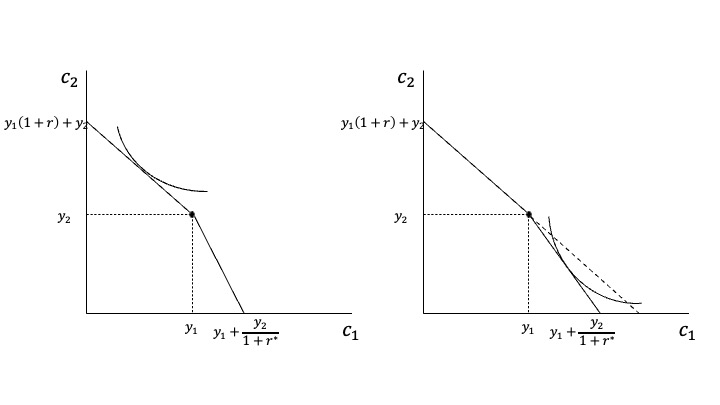
\includegraphics[width=\textwidth]{Figuras/CI Restricciones de liquidez.jpeg}
    \label{fig: Restricciones liquidez bienestar}
\end{figure}

Podemos ver los efectos en el bienestar de un consumidor bajo restricciones de liquidez en dos casos. Uno en el cual el consumidor prefiere ahorrar, en este caso se dice que la restricción no está activa puesto que las restricciones de liquidez solo afectan a la tasa de endeudamiento (Figura \ref{fig: Restricciones liquidez bienestar}). El caso en que el individuo preferiría endeudarse, en estas condiciones la restricción está activa, el punto que maximizaba el bienestar ya no es factible y por tanto hay una perdida en cuanto a utilidad. 

Es fácil ver que las restricciones tienen efectos negativos (o nulos) en el bienestar de las personas pues reduce la cantidad de opciones factibles en las que maximizar utilidad. 

\section{Inconsistencia temporal}

\section{Optimización interestados y la aversión al riesgo}

\section{Seguros}

\input{Tex/La teoría de mercados eficientes}

\section{La teoría de la protección social}

\section{Trampas de impaciencia y trampas de miedo}

\begin{appendices}
\chapter{Apéndice}

\section{Random Walk}

Incluyendo incertidumbre a un modelo con expectativas racionales podemos obtener distintos resultados dependiendo del tipo de función de utilidad. En este caso veremos como un individuo neutro al riesgo sigue una trayectoria de consumo tipo \textit{random walk}.

Primero resolvamos el problema con un consumo futuro incierto.
\begin{align*}
    \max _{c_t , c_{t+1}} \quad  u(c_t)+ \mathbb{E}_t \{u(c_{t+1})\} \\ 
    s.a \quad y_t + \frac{y_{t+1}}{1+r} = c_t +\frac{c_{t+1}}{1+r}
\end{align*}

Planteamos el lagrangeano:
\begin{equation*}
    \mathcal{L}: u(c_t)+ \mathbb{E}_t \{ u(c_{t+1}) \} + \lambda \left(y_t + \frac{y_{t+1}}{1+r} - c_t - \frac{c_{t+1}}{1+r} \right)
\end{equation*}

Derivamos las condiciones de primer orden para encontrar la ecuación de Euler del consumo. 
\begin{align}
    \frac{\partial \mathcal{L}}{\partial c_t} =u'(c_t) -\lambda = 0    \notag \\   u'(c_t) = \lambda \\
    \frac{\partial \mathcal{L} }{\partial c_{t+1}} = \frac{1}{1+\rho} \mathbb{E}_t \{ u'(c_{t+1})\} - \frac{\lambda }{1+r} = 0 \notag 
 \\ \frac{1+r}{1+\rho } \mathbb{E}_t \{u'(c_{t+1})\} = \lambda \\
 u'(c_t) = \frac{1+r}{1+\rho} \mathbb{E}_t\{u'(c_{t+1})\} \label{eq: Ecuación de euler random}
\end{align}

La expresión \ref{eq: Ecuación de euler random} es la ecuación de Euler.

Para probar que un individuo neutral al riesgo sigue un \textit{random walk} en este caso podemos reemplazar la función de utilidad con una función cuadrática como en la expresión \ref{eq: ecuación cuadrática}. La utilidad marginal por tanto va a ser lineal lo cual describe un individuo neutro al riesgo.
\begin{equation}
    u(c_t) = bc_t - \frac{a}{2}c_t ^2 \label{eq: ecuación cuadrática}
\end{equation}

Remplazmaos las funciones de utilidad marginales en la ecuación de Euler del consumo y asumimos que $r=\rho = 0$:
\begin{align*}
    b-ac_t = \mathbb{E}_t\{b-ac_{t+1}\}
\end{align*}

Aplicamos propiedades de la esperanza y simplificamos los $b$ y $-a$:
\begin{equation}
    c_t = \mathbb{E}_t \{c_{t+1} \} \label{eq: random walk resultado}
\end{equation}
Según muestra la ecuación \ref{eq: random walk resultado} el consumo en $t$ va a ser igual a lo que se espera que sea el consumo en $t+1$. Por lo que la trayectoria de consumo se mantendrá igual hasta que llegue un shock que la desvíe.

\section{Incertidumbre y ahorro por precaución}

Bajo el mismo caso de incertidumbre, un individuo con aversión al riesgo tendrá un ahorro por precaución. Esto ya que no se cumple el caso de \ref{eq: random walk resultado} ya que tendremos utilidades marginales crecientes a tasas decrecientes. 

Esto se traduce en que la esperanza de la utilidad es mayor a utilidad de la esperanza
\begin{equation}
    \mathbb{E}_t \{ u(c_t) \} < u(\mathbb{E}_t \{ c_t \})
\end{equation}
Podemos derivar la expresión. 
\begin{equation}
    \mathbb{E}_t \{ u'(c_t) \} > u'(\mathbb{E}_t \{ c_t \})
\end{equation}
Según \ref{eq: Ecuación de euler random} (con $\rho = r = 0$) podemos reemplazar.
\begin{align}
    u'(c_t) = u'(\mathbb{E}_t \{ c_{t+1} \}) < \mathbb{E}_t\{ u'(c_{t+1}) \} \notag \\
    u'(c_t) < \mathbb{E}_t\{ u'(c_{t+1}) \} \label{eq: incertidumbre marginla averso}
\end{align}
De \ref{eq: incertidumbre marginla averso} podemos interpretar que debido al perfil del consumidor se consume menos por una necesidad de ahorro por precaución.

\section{Modelo CAPM de consumo}
Los retornos están sujetos a varianza. retornos puedes estar sujetos a varianza (incertidumbre). Para individuos con expectativas racionales que tienen la opción de consumir en el presente o de invertir para llevar dinero al futuro podremos llegar a la ecuación de euler del tipo \ref{eq: Ecuación de euler random}. Específicamente,
\begin{equation}
    u'(c_1) = \mathbb{E}_1  \left[  \frac{1+r^i}{1+\rho} u'(c_2)  \right] \label{eq: Ecuación de euler random 2}
\end{equation}
Donde $r^i$ es un activo con riesgo. Queremos buscar el diferencial entre la esperanza del activo riesgoso y el libre de riesgo. Utilizando las propiedades de la esperanza podemos desarrollar sacando el descuento intertemporal de la esperanza y multiplicando la esperanza de los retornos $1+r^i$ y $u'(c_2)$. Recordamos como desarrollar $\mathbb{E}(X\cdot Y)$ y aplicamos a \ref{eq: Ecuación de euler random 2}
\begin{align}
    \mathbb{E}(X\cdot Y) = \mathbb{E}(X) \cdot \mathbb{E}(Y) + \text{Cov}(XY) \\
    u'(c_1) = \frac{1}{1+\rho} \left[ \mathbb{E}_1(1+r^i) \cdot \mathbb{E}_1 (u'(c^2)) + \text{Cov}(1 + r^i, u'(c_2)       \right] \\
    \mathbb{E}_1 (1+r^i) = \frac {1}{\mathbb{E}_1 (u'(c_2))} \left[   (1+\rho)u'(c_1) - \text{Cov}(1+r^i, u'(c_2))     \right] \label{eq: Diferencial riesgoso}
\end{align}

Ahora tenemos la esperanza de los activos riesgosos, necesitamos encontrar el diferencial entre estos y los de libre riesgo. Sabemos que en caso de que $1+r$ sea libre de riesgo podremos sacar los retornos como constantes de  \ref{eq: Ecuación de euler random 2}. Llegamos a lo siguiente,
\begin{equation}
    1+r = \frac{1}{\mathbb{E}_1 (u'(c_2))} [(1+\rho)u'(c_1)] \label{eq: diferencial libre de riesgo}
\end{equation}
Por lo que ahora que tenemos las variables definidas podemos encontrar el diferencial restando \ref{eq: Diferencial riesgoso} con \ref{eq: diferencial libre de riesgo}. 
\begin{equation*}
    \mathbb{E}_1 (1+r^i) - (1+r) = \frac {(1+\rho)u'(c_1) - \text{Cov}(1+r^i, u'(c_2)) - (1+\rho)u'(c_1) }{\mathbb{E}_1 (u'(c_2))}  
\end{equation*}
Llegamos a que la diferencia entre los retornos riesgosos y los libres de riesgos debieran seguir esta igualdad.
\begin{equation}
    \mathbb{E}_1(r^i) - r = - \frac{\text{Cov}(1+r^i, u'(c_2))}{\mathbb{E}_1(u'(c_2))}
\end{equation}
Esta expresión es la que da sentido a los premios por riesgo de un activo con retornos inciertos. Aunque se parezca mucho al consumo intertemporal este modelo CAPM de consumo considera incertidumbre. Por lo que las personas no solo estarían decidiendo si invertir a futuro por precaución sino también por aumentar el consumo futuro bajo un riesgo. 

En caso de que si $\text{Cov}(1+r^i,u'(c_2))<0$ habrá un premio de por riesgo. Recordando que $u'(c_2)<0$ podemos inferir que el retorno covaría positivamente con el consumo, por lo que en el futuro $t=2$ se necesitaría pagar un premio por riesgo. Esto ya que si un activo paga más cuando el consumo es alto no estaría proveyendo de un seguro contra las caídas del ingreso, la única razón de mantenerlo en el portafolio sería si provee un buen retorno. 

En caso de que $\text{Cov}(1+r^i,u'(c_2))>0$, es decir el retorno es bajo cuando el consumo es alto el rendimiento será menor al libre de riesgo. Esto es porque además de servir como ahorro también juega una función de seguro contra los malos tiempos

% desarrollar mejor, esto está en los ppt de macroeconomía I y falta mucho detalle...

% Introducir de mejor manera el capm
\end{appendices}

% Creo provisoriamente este capítulo para incluir apuntes de organización industrial que pueden ser utiles para otras secciones
\chapter{Organización industrial}

\input{Tex/Teoría de juegos.tex}

\section{Competencia imperfecta}

\subsection{El factor estratégico}

Los \textbf{oligopolios},\marginnote{\textbf{Oligopolio:} Mercado con un número reducido de firmas las cuales pueden incidir en el precio.}[0cm] también llamados mercados de competencia imperfecta, son un escenario en el cual un número reducido de empresas inciden en cierta medida en el precio de mercado. Es por esto que se le considera un entremedio entre monopolio y competencia perfecta, no eligen libremente pero tampoco son tomadores de precio. 

Todas las firmas tienen cierto poder sobre el precio de mercado, directamente fijando los precios o indirectamente decidiendo las cantidades a producir. Debido a que todas las firmas afectan el precio habrá \textbf{interdependencia monopolística},\marginnote{\textbf{Intedependencia monopolística:} De manera más general llamado interdependencia estratégica. Las empresas toman sus decisiones formando creencias de lo que hará su competencia.}[-1cm] lo cual sugiere que hay un factor estratégico en las competencias olipólicas. Por ejemplo, si una firma fija cierto precio, su rival puede responder con un precio menor para quedarse con una mayor demanda.\footnote{Esto asumiendo que son bienes perfectamente sustitutos (producto homogéneo).} También, si se cree que la firma rival va a producir mucho del bien, a las demás firmas les conviene producir menos para no desplomar el precio de mercado por un exceso de oferta. Es decir, las decisiones de una firma afectan a su competencia y viceversa, ante esto las firmas formarán creencias de lo que hará la competencia para tomar sus propias decisiones. 

\subsubsection*{La estrategia desde la teoría de juegos}

La manera en que entendemos estas interacciones propias de la \textbf{organización industrial}\marginnote{\textbf{Organización industrial:} Área de la teoría de la firma que se enfoca en la estructura e interacciones en los mercados.} es mediante la teoría de juegos. Tal como se mencionaba antes, en la teoría de juegos los jugadores tienen que formar una creencia de lo que hará el otro para reaccionar de la mejor manera. A continuación plantearemos como se verían estos juegos aplicado a los distintos tipos de competencia imperfecta. 

Para esta ocasión solo se abarcarán juegos normales, es decir, los jugadores $i \in 1,2,\ldots,N$ serán racionales y deciden su acción o combinación de acciones $a_i \in A_i$ resultando en un pago $\pi_i(a)$ para cada firma.

Las firmas elegiran $a_i$ de manera de maximizar sus pagos, una estrategia será mejor que otra mientras el pago resultante sea mayor. Dado que los rivales $-i$ escogen una estrategia $a_{-i}$, la firma $i$ tendrá una respuesta óptima $a_i^*$ en que los pagos sean mayores, es decir,\footnote{Dada las características del juego y considerando que los individuos son racionales es esperable que siempre elijan la respuesta óptima $a_i^*$.} 
\begin{equation}
    \pi_i(a_i^*, a_{-i}) \geq \pi_i(a_i, a_{-i}), \forall a_i . \label{eq: mejor respuesta}
\end{equation}
Esto es equivalente a decir que jugando piedra papel o tijera, si mi rival elige tijera la mejor respuesta para el papel es la tijera, mientras que la mejor respuesta para la tijera es la roca. Podremos describir matemáticamente la mejor respuesta de $i$ en función de la estrategia de los demás; $a^*_i(a_{-i})$. A esto se le conoce como \textbf{función de reacción}.\marginnote{\textbf{Función de reacción:} Función que describe la mejor forma de responder ante las decisiones de un competidor.} Cuando todas las firmas elijan su mejor estrategia $a^* \equiv (a_1^*,\ldots,a_N^*)$ no habrán incentivos a cambiar de estrategia, por lo que nos encontraríamos en el Equilibrio de Nash.\footnote{En el caso de piedra papel o tijeras no habría Equilibrio de Nash, suponiendo que todas las opciones tienen las misma probabilidad de ser elegidas.} 

Las firmas seguiran esta manera de pensar para decidir que tienen que hacer al competir con otra firma. En el corto plazo las firmas suelen tomar acciones respecto a la fijación de precios o al nivel de producción, en el largo plazo se podría hablar de entradas a mercado o de inversión en I+D, etc. Veremos a continuación dos modelos que discuten tipos de competencia por precios y cantidades.

\subsection{Competencia a la Bertrand}

\subsubsection{Planteamiento}
Este modelo fue planteado por el matemático \textbf{Joseph Bertrand}\marginnote{\textbf{Joseph Bertrand (1822-1900):} Matemático francés del siglo XIX. Proporcionó aportes a la economía como fue el modelo de Bertrand. Fue crítico del principio de maximización de utilidad.}[0cm] en 1883. Vamos a pensar en un duopolio de firmas $i\in 1,2$ que ofrecen un producto homogéneo compitiendo precios $p_i$. 

Como los productos son homogéneos, es decir son sustitutos perfectos, la firma que ofrezca el menor precio se llevará toda la demanda $Q_i(p_i)$, en caso de ofrecer un mismo precio se reparten la demanda de manera equitativa. Por lo demás, las firmas tendrán un costo marginal $c_i$. 

Para entender como se llega al equilibrio en este mercado primero tenemos que identificar cuales son las mejores respuestas de una firma ante acciones de la otra, es decir la $a^*_i(a_{-i})$. Pensando desde el punto de vista de la firma $1$ podemos considerar 3 casos posibles y sus respectivas respuestas ante acciones de la firma $2$, buscamos definir la función de reacción $p^*_1(p_2)$.

\begin{itemize}
    \item En caso de que la firma $2$ fije un precio $p_2$ mayor al precio monopólico $p_1^M$. La mejor respuesta es fijar el precio monopólico, de esta manera maximizan beneficios mientras absorben toda la demanda.
    \item Si la firma $2$ fija un precio menor al precio monopólico $p_1^M$ y mayor a al costo marginal $c_1$. Para capturar toda la demanda conviene fijar un precio minúsculamente menor al de la competencia, lo cual se denota como $p_1-\epsilon$ siendo $\epsilon$ un número positivo cercano al cero.
    \item La firma $2$ fija un precio igual o menor al costo marginal $c_1$. Para estos casos la mejor respuesta es fijar el costo marginal.
\end{itemize}

El precio $p_1$ que fije la firma $1$ en función de $p_2$ puede ser descrito en esta función y representado en la figura \ref{fig:funciones de reacción Bertrand},
\begin{align*}
    p^*_1(p_2)= \left\{ \begin{array}{lcc} p_1^M & \text{si} &  p_2> p_1^M \\ \\ p_2-\epsilon & \text{si} & p_1^M \geq p_2>c_1 \\ \\ c_1 & \text{si} & c_1 \geq p_2 \end{array} \right.
\end{align*}

\begin{figure}[htb]
    \centering
    \caption{Funciones de reacción de competencia tipo Bertrand con firmas simétricas}
    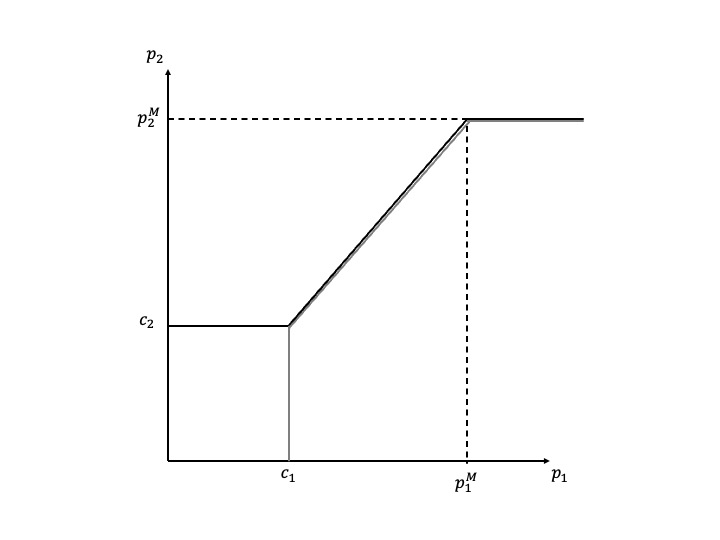
\includegraphics[width=15cm]{Figuras/Función de reacción Bertrand.jpeg}
    \label{fig:funciones de reacción Bertrand}
\end{figure}


\subsubsection{Equilibrios de competencia a la Bertrand}

Un caso útil para describir la dinámica se da cuando las empresas son simétricas, lo cual implica que tienen un mismo costo marginal $c$. La dinámica aquí es que la mejor respuesta ante cualquier precio $p_{-i}^M \geq p_i>c$ será fijar un precio menor, ante lo cual la competencia debería responder con un precio aun menor. De esta manera el precio bajará hasta el punto en que tanto $p_1$ como $p_2$ sean iguales a $c$. 

Este caso es conocido como la \textbf{paradoja de Bertrand}.\marginnote{\textbf{Paradoja de Bertrand:} Durante la competencia de un duopolio con firmas simétricas el equilibrio de Nash se da donde el precio es igual al costo marginal. Es decir, se llega al resultado de competencia perfecta con sólo 2 firmas.}[-3.5cm] Se le da este nombre puesto que el resultado de esta competencia imperfecta con 2 firmas es el mismo que en competencia perfecta ($p=c$). Tal como se ve en la figura \ref{fig:EN Bertrand sim}. 

\begin{figure}[htb]
    \centering
    \caption{Equilibrio de Nash en Bertrand con firmas simétricas}
    \includegraphics[width=15cm]{Figuras/EN Bertrand con firmas simétricas.jpeg}
    \label{fig:EN Bertrand sim}
\end{figure}

El resultado de una competencia en que una firma es más eficiente dista de lo anterior. Cuando una firma tiene un costo marginal menor a su rival podrá absorber toda la demanda fijando un precio ligeramente menor al costo marginal de su competencia. Más precisamente en el caso en que $c_1<c_2$ el equilibrio resulta en $p_1 = c_2 - \varepsilon$. Lo cuál llevaría a la firma menos eficiente a salir del mercado y la firma ganadora obtendría beneficios. Vease \ref{fig:EN Bertrand asim}. 

\begin{figure}[htb]
    \centering
    \caption{Equilibrio de Nash en Bertrand con firmas asimétricas}
    \centering
    \includegraphics[width=15cm]{Figuras/EN Bertrand firmas asimétricas.jpeg}
    \label{fig:EN Bertrand asim}
\end{figure}

\subsection{Competencia a la Cournot}

\subsubsection{Planteamiento}

Otra manera de modelar la competencia entre firmas $i \in 1,2$ es mediante las cantidades de producción de cada una, lo cual se puede extrapolar a mercados con nula diferenciación de producto (Nuevamente nos referimos a productos homogéneos).\footnote{Por ejemplo, no importa la marca del cobre, no hay diferenciación de producto. El mayor predictor del precio asumiendo fija la demanda será la oferta.} El matemático francés \textbf{Antoine Cournot}\marginnote{\textbf{Antoine Cournot (1801-1877):} Filósofo y matemático frances que impulso la economía marginalista. Fue de los primeros quienes empezaron a usar funciones matemáticas para describir relaciones como la oferta y la demanda}[-4.5cm] planteó un modelo de mercado de un bien homogéneo donde la única variable estratégica que manejan las firmas es el nivel de producción.

Presentaremos el modelo dentro de un duopolio en donde cada firma produce una cantidad $q_i$, donde el total producido $Q$ es la suma de las producciones individuales.
\begin{equation}
    Q = \sum_{i=1}^N q_i = q_1 + q_2 + \ldots +q_N
\end{equation}
Asumiremos que las firmas son simétricas (mismo costo marginal) y enfrentan una misma demanda inversa lineal $P(Q) = A - Q$. 

Para resolver el modelo debemos de plantear el problema que enfrenta cada firma. Esto es, maximizar beneficios considerando lo que pueden producir y vender $q_i$ y el beneficio marginal de cada producto $P-c$.
\begin{equation}
    \max_{q_i} \quad \Pi _i = (P-c)q_i \label{eq: maximización}
\end{equation}
Como todas las producciones de distintas empresas están contenidas en \ref{eq: maximización} mediante el precio,\footnote{De la manera $P = A-\sum_{i = 1}^Nq_i$.} al optimizar obtendremos la cantidad que debiera producir la firma para maximizar sus beneficios en función de las decisiones de su competencia. Esto es, la estrategia óptima $q_i^*$ ante la estrategia del rival $q_j$. Resolvemos para la firma $1$.
\begin{align*}
\max_{q_1} \quad \Pi_1 &= (P-c)q_1 = (A-q_1-q_2)q_1 - cq_1 \\
\text{CPO:} \quad \frac{\partial \Pi_1}{\partial q_1} &= A-2q_1 - q_2 -c =0
\end{align*}
Teniendo las condiciones de primer orden solo queda despejar para obtener la función de reacción de la firma $1$ ante la estrategia de la firma $2$.
\begin{equation}
    q^*_1(q_2) = \frac{A-q_2-c}{2} \label{eq: Función de reacción 1}
\end{equation}

La mejor estrategia para $1$ dependerá de la producción de $2$. La producción óptima $q^*_1$ bajará en caso de que el rival produzca más $\Delta^+ q_2$, esto ya que aumentar la producción causaría que el precio caiga más de lo ideal por el exceso de oferta. Es por esto que en competencias a la Cournot la pendiente de la función de reacción será negativa.\footnote{En Bertrand hay pendiente positiva en ciertas partes de la función puesto que un aumento de precio de una firma no llevaba a una reducción del precio de la otra.}

\subsubsection{Equilibrio de competencia a la Cournot} 

Recordemos que las firmas llegarán a un equilibrio de Nash cuando estas respondan su estrategia óptima ante la estrategia óptima de sus competidoras. Dadas las funciones de reacción es trivial encontrar el equilibrio, directamente se reemplaza la función de respuesta $q^*_2(q_1)$ en $q^*_1(q_2)$ o viceversa.

\begin{figure}[htb]
    \centering
    \caption{Equilibrio de Nash en Cournot}
    \centering
    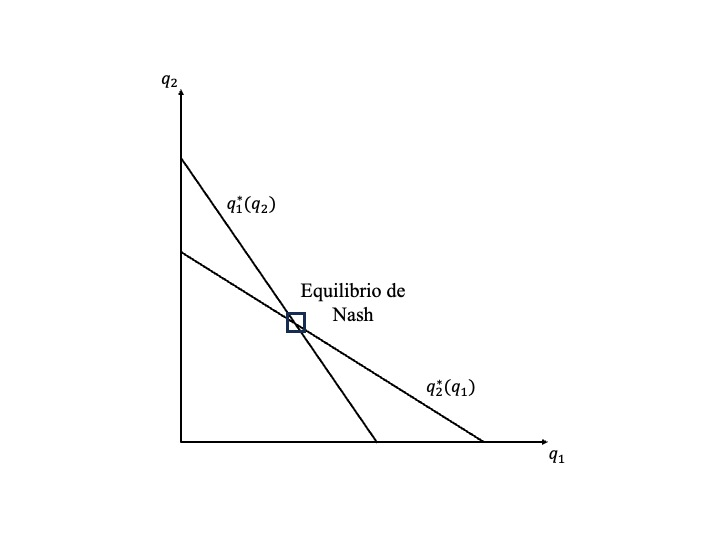
\includegraphics[width=12cm]{Figuras/EN Cournot.jpeg}
    \label{fig:EN Cournot}
\end{figure}

Como en este caso las firmas son simétricas podemos decir que $q_1 = q_2 = q$ y resolver directamente. 
\begin{align}
    q &= \frac{A-q-c}{2} \notag \\
    q &= \frac{A-c}{3} \label{eq: producción individual}
\end{align}
Según \ref{eq: producción individual} tendremos la producción individual de las dos firmas.

El precio se determinará por el total de oferta en el mercado, es decir, la producción de cada una de las firmas $Q = 2q$. 
\begin{align}
    P &= A-2 \cdot \left( \frac{A-c}{3} \right) \notag \\
    P &= \frac{A-2c}{3}
\end{align}
Por último podemos determinar los beneficios de cada firma reemplazando los valores en \ref{eq: maximización}
\begin{align}
\Pi_i &= \left(\frac{A-2c}{3}-c \right) \frac{A-c}{3} \notag \\ 
\Pi_i &= \frac{(A-c)^2}{9}
\end{align}

Este ejemplo de equilibrio es con firmas simétricas, en caso de haber una firma más eficiente a esta le convendría producir más. Graficamente la empresa más eficiente debiera tener una función de reacción más desplazada hacia la derecha. 

\subsubsection*{Caso para $n$ firmas}
Como ejercicio se recomienda hacer este mismo procedimiento para $n$ firmas en el mercado. Una vez hecho se recomienda analizar los efectos marginales de aumentos o reducciones en $n$ y el caso en que $n$ tiende a infinito.


\section*{Recapitulación y observaciones}

En los dos tipos de competencia las firmas forman creencias de lo que hará la competencia para poder maximizar beneficios. En el caso de Bertrand presentado la solución es directa y no se requiere de plantear el problema de maximización de beneficios. 

Se puede notar mirando los beneficios en cada caso, que competir a la Bertrand es mucho más competitivo que a la Cournot. Una empresa más eficiente que su competencia en Cournot podrá vender más, en Bertrand se quedará con todo el mercado. 

En los casos presentados se supone implícitamente que las empresas tienen capacidad de servir a todo el mercado que quieran. Este supuesto no es realista y se puede levantar dando pasos a otras conclusiones pero que no se desvían mucho de lo ya visto. Se puede encontrar más detalle en el anexo. 

\subsection{Competencia a la Stackelberg}

Este modelo fue propuesto por el economista alemán \textbf{Heinrich von Stackelberg}.\marginnote{\textbf{Heinrich von Stackelberg (1905-1946)}: Economista alemán de ascendencia argentina nacido en Rusia, arrepentido miembro del Partido Nazi y sargento de la SS, falleció en España. Aportó a la teoría de juegos.}[0cm] Ya habiendo comprendido el modelo Cournot no es complejo entender el modelo Stackelberg.\footnote{Competencia a la Stackelberg es una tipo de competencia a la Cournot.} El \textit{twist} con respecto al modelo anterior se encuentra en que las firmas jugarán por turnos, inevitablemente la primera a jugar tiene la ventaja. 

Supongamos que la firma $1$ es la líder pues juega primero, mientras que la firma $2$ es la seguidora. La firma líder decidirá en el $t = 1$ la cantidad $q_1$ que producirá y en $t=2$ la firma seguidora decidirá su producción $q_2$ en función de $q_1$.

Este tipo de juegos se tienen que resolver por inducción. Si miramos el problema desde el final hasta el inicio primero se maximizan los beneficios de la firma $2$, la cual en $t = 2$ ya sabrá qué produjo la firma $1$, de lo cual obtendremos $q_2^*(q_1)$. La firma líder tendrá que maximizar en $t=1$ sujeto a lo que hará la seguidora en $t=2$. El problema de la firma $1$ se plantea de la siguiente manera,
\begin{align*}
    \max_{q_1} \quad &\Pi_1 = (P(Q)-c)q_1 \\
    \text{s.a}\quad &q_2=q_2^*(q_1)
\end{align*}
Suponiendo una demanda lineal y que las firmas son simétricas podemos considerar (\ref{eq: Función de reacción 1}) como la función de reacción para la firma seguidora. Reemplazamos la restricción en la expresión a maximizar y reescribimos el problema como,
\begin{align*}
    \max_{q_1} \quad &\Pi_1 = \left(A-q_1-c- \left(\frac{A-q_1-c}{2} \right) \right)q_1 \\ & \Pi_1 = \left( \frac{A-q_1-c}{2}   \right)q_1 \\
    \text{CPO:} \quad & \frac{\partial \Pi_1}{\partial q_1} =   \frac{A-c}{2} -q_1 = 0 \\
    & q_1 = \frac{A-c}{2}
\end{align*}
Reemplazando $q_1$ en $q_2^*(q_1)$ obtendremos la producción de la firma seguidora. 

La producción de la firma líder aumenta por sobre el caso de Cournot con turnos simultáneos. La firma líder tiene más espacio para aumentar la producción para aumentar ventas, mientras que la seguidora tendrá que adaptarse produciendo menos para que el precio no baje demasiado.


\section{Acuerdos colusivos}

Como se puede notar en el problema de la firma, cada empresa maximiza los beneficios propios y no los conjuntos, lo cual es un factor en el nivel competitivo de las firmas y el poder de mercado que ostenten. Sin embargo, la competencia no es buena para las firmas, al haber más firmas lo esperable es que el precio vaya convergiendo al costo marginal, lo cual muestra como van perdiendo poder de mercado. La colusión es una manera en que las firmas se compromoten a colaborar para aumentar las utilidades personales. 

En la realidad se ven distintos tipos de colusiones las cuales dependiendo el producto tomarán diferentes formas; Aumento de precios, reducción de oferta, restricciones territoriales y mecanismos de castigo. Es útil para las instituciones fiscalizadores estudiar y comprender los factores que podrían indicar una colusión o que faciliten un acuerdo colusivo. 

La teoría de juegos nos ayuda a modelar las decisiones de las firmas mediante \textbf{juegos iterativos}.\marginnote{\textbf{Juegos iterativos:} Juegos en los cuales hay más de un período/turno en que se juega. Pueden ser finitos e infinitos.}[-3cm] Sin embargo hay que considerar un punto muy importante, en caso de períodos finitos no es posible el \textbf{equilibrio perfecto en subjuegos}\marginnote{\textbf{Equilibrio perfecto en subjuegos:} En los juegos dinámicos de información perfecta habrá un equilibrio perfecto en subjuegos cuando se de un equilibrio por inducción en donde todas las decisiones sean creíbles.} colusivo, sólo será posible en iteraciones infinitos lo cual se explicará más adelante.

En este tipo de acuerdos habrá un incentivo a traicionar, es decir, desviarse del acuerdo para conseguir incluso mayores utilidades de las que conseguirían coludiéndose. En caso de que esto ocurra las demás empresas seguirán una \textbf{estrategia gatillo}, provocando que se acabe la fase de colaboración y empiece la fase de castigo. El castigo es empezar a competir normalmente por el resto del juego, ya sea a la Bertrand, Cournot, etc.

En los casos finitos de $T$ períodos de tiempo nunca habrá incentivos para cooperar en el último período. Como no hay un mañana $T+1$ no habría fase de cástigo por desviarse en $T$, todos preferiran traicionarse el uno al otro. En $T$ nadie coopera lo cual induce a que nadie coopere en $T-1$, el resultado es que nadie coopera en ninguno de los períodos. Nunca hay colusión con períodos finitos, mientras que existen equilibrios colusivos en $T$ infinitos cumpliendose ciertas condiciones. Una empresa se coludirá perpetuamente en caso de que los beneficios de coludirse sean mayores a los de no hacerlo. 

\subsection*{Planteamiento}

Las firmas al coludirse estarán ponderando si es que los beneficios de traicionar en el corto plazo compensarán los beneficios de mantenerse coludidos en el largo plazo. Si una firma se desvía quiere decir que en ese turno gana los beneficios extraordinarios $\pi^D$, los cuales suelen ser los beneficios monopólicos $\pi^M$, durante los siguientes turnos por estrategia gatillo todos empiezan a competir obteniendo en este caso $\pi^G$.\footnote{$\pi^G$ va a depender del las condiciones del mercado, demanda, competidores, tipo de competencia; Cournot, Bertrand, Stackelberg, etc.}

Además se tiene que considerar que los beneficios de períodos más lejanos al presente tendrán menos peso para las decisiones de las firmas. De manera similar al modelo de consumo intertemporal vamos a ponderar los períodos futuros por un descuento $0 \leq \delta < 1$ para todos los períodos $t \in 0,1,2,\ldots,T$.

\subsubsection*{Condición de colusión para Bertrand}

Vamos a ver un caso específico para introducirnos en la dinámica. En el caso de un duopolio Bertrand con firmas simétricas ($\pi^G=0$ y $\pi^D = \pi^M$) podemos describir los beneficios de desviarse $V^D$ en el período $t=0$ como,\footnote{El factor $\frac{\delta}{1-\delta}$ viene de la suma geométrica.}
\begin{equation}
    V^D = \delta^0 \pi^M + \delta \pi^G + \delta^2 \pi^G+ \ldots + \delta^T \pi^G= \pi^M + \frac{\delta}{1-\delta} \pi^G = \pi^M \label{eq: Desvío del acuerdo competencia a la bertrand}
\end{equation}
\ref{eq: Desvío del acuerdo competencia a la bertrand} denota las utilidades de desviarse y obtener beneficios monopólicos en el primer turno y luego competir a la Bertrand obteniendo cero beneficios. En caso de seguir la colusión calculamos $V^C$ como el reparto de las utilidades monopólicas $\frac{\pi^M}{N}$. 
\begin{equation}
    V^C = \delta^0 \frac{\pi^M}{2} + \delta ^1 \frac{\pi^M}{2} + \delta ^2 \frac{\pi^M}{2} +\ldots + \delta^T \frac{\pi^M}{2} = \frac{\pi^M}{2} + \frac{\delta}{1-\delta} \frac{\pi^M}{2}
\end{equation}
La colusión se dará cuando para cada empresa se cumpla que, 
\begin{equation}
    V^C \geq V^D
\end{equation}
Para evaluar si esto ocurre tendremos que fijarnos que la tasa de descuento $\delta$ cumpla ciertas condiciones,
\begin{align*}
    V^C \geq V^D \Longleftrightarrow \frac{\pi^M}{2} + \frac{\delta}{1-\delta} \frac{\pi^M}{2} \geq \pi^M \\
    \text{Despejando $\delta$ obtenemos la condición} \quad \delta \geq \frac{1}{2}
\end{align*}

Es decir, mientras se cumpla que $\delta \geq \frac{1}{2}$ el acuerdo colusivo se va a dar en todos los períodos. La interpretación es que si las firmas tienen un nivel de paciencia suficientemente alto para valorar los beneficios de coludirse a largo plazo, preferiran mantener el acuerdo antes de los beneficios de corto plazo del desvío. 

\subsubsection*{Colusiones, caso general}

Una fórmula general de expresar lo anterior es la siguiente,
\begin{equation}
    \frac{\delta }{1-\delta} (\pi ^C - \pi^{G}) \geq \pi ^D- \pi^C \label{eq: Condición de colusión generalizada}
\end{equation}

Donde $\pi^C$ serán los beneficios que recibe la empresa al coludirse con las demás,\footnote{Nótese que es diferente a $\pi^M$ puesto que se tienen que repartir entre las firmas coludidas.} $\pi^D$ son los beneficios del turno al desviarse y $\pi^G$ serán los beneficios donde por estrategia gatillo todas las firmas empiecen a competir. \ref{eq: Condición de colusión generalizada} se interpreta como que los beneficios a largo plazo deben ser más valorados que los beneficios a corto plazo. 

De \ref{eq: Condición de colusión generalizada} también podemos despejar el descuento $\delta$. De esta manera conseguiremos el $\delta$ mínimo para asegurar que la colusión se cumpla.
\begin{equation}
    \delta \geq \frac{\pi^D - \pi ^C}{\pi^D- \pi^G} \label{eq: Condición que tiene un nombre del que no me acuerdo ;(}
\end{equation}

\subsection{Factores que facilitan o dificultan la colusión}

Hay distintos factores que pueden facilitar la colusión, el factor de descuento es uno de ellos. Derivaremos los siguientes factores:
\begin{itemize}
    \item A mayor cantidad de firmas más díficil es mantener un equilibrio colusivo.
    \item Ante una fase de castigo más severa es sea más fácil mantener la colusión.
    \item En caso de asimetría en las firmas, habrá quienes sean más propensas o menos propensas a mantener el trato.
\end{itemize}

\subsubsection*{Cantidad de firmas y acuerdos colusivos}

Para un número de $N$ firmas iguales compitiendo a la Cournot las utilidades de coludirse bajaran con la cantidad de firmas, $\pi^C = \frac{\pi^M}{N}$. Si en un turno una firma se desvía ganan $\pi^M$, para simplificar diremos que en la fase de castigo $\pi^G = 0$.

Citando \ref{eq: Condición que tiene un nombre del que no me acuerdo ;(} y reemplazando los beneficios para este caso obtenemos el descuento mínimo necesario para que la colusión sea posible $\bar{\delta}$. 
\begin{align*}
    \delta \geq \frac{\pi^M - \frac{\pi^M}{N}}{\pi ^M - 0} \Longleftrightarrow &\bar{\delta} = 1 - \frac{1}{N} \\
    & \frac{\partial \bar{\delta}}{\partial N} > 0
\end{align*}

A mayor cantidad de firmas es más difícil que las empresas se coludan pues requieren ponderar en mayor medida los beneficios a largo plazo del acuerdo. Es por esto que las instituciones fiscalizadores ponen especial atención en mercados con pocas firmas. 

\subsubsection*{Fases de castigo y acuerdos colusivos}

Es intuitivo pensar que si el castigo es mayor es más fácil alcanzar un acuerdo colaborativo. Anteriormente se mencionó como Bertrand es un tipo de competencia más fuerte que Cournot, lo cual conlleva que sea más fácil llegar a acuerdos colusivos en Bertrand que en Cournot. Esto se puede ver directamente en la expresión \ref{eq: Condición que tiene un nombre del que no me acuerdo ;(}, competir a la Cournot suele resultar en que $\pi^G$ sea mayor que en Bertrand. 
\begin{align*}
    \frac{\partial \bar{\delta}}{\partial \pi^G} > 0
\end{align*}

Al haber menos castigo es necesaria mayor paciencia para mantener el acuerdo. 

\subsubsection*{Asimetría en las firmas y acuerdos colusivos}

Un punto muy relacionado a lo anterior es el tema de acuerdos colusivo entre firmas asimétricas. En un acuerdo la firma más eficiente tendrá una suerte de dominancia por sobre la otra puesto que en caso de competir la más eficiente saldrá mejor parada. Es por lo anterior que las firmas más eficientes requerirán de mayor paciencia mínima $\bar{\delta}$ para mantener el acuerdo. 

\begin{appendices}
    \chapter{Anexo}

\section{Cournot con restricciones de capacidad}

De forma complementaria se puede levantar el supuesto de que una sola empresa podría servir a todo el mercado si así lo quisiera. Algo más parecido a la realidad es que una sola firma no puede servir a todo el mercado aunque así lo quisiera. La capacidad de una firma puede denotarse como $K$. Frente a una demanda inversa lineal $P(Q) = A-Q$ y considerando dos firmas idénticas de $c=0$ tendremos restricciones activas de capacidad en caso de que $K \leq A$. 

En caso de que compitan la pregunta es qué parte de la curva de demanda sirve cada firma. Se puede asumir racionamiento eficiente, en caso de haber dos precios distintos el más barato será el primero en venderse a los que están más dispuestos a pagar. Una vez vendida toda la capacidad de la firma más barata la otra firma se queda con el sobrante.
\end{appendices}


\end{document}